\documentclass[11pt,multicol]{article}

\usepackage{amsmath}
\usepackage{amssymb}
\usepackage{multicol}
\usepackage{booktabs}
\usepackage{color}
\usepackage{epigraph}
\usepackage{float}
\usepackage{fourier}
\usepackage{fullpage}
\usepackage{fullpage}
\usepackage{graphicx}
\usepackage{listings}
\usepackage{subcaption}
\usepackage{url}
\usepackage{wrapfig}
\usepackage{xspace}
\usepackage[colorlinks=true,urlcolor=blue]{hyperref}

\usepackage{fancyhdr}
\pagestyle{fancy}
\fancyhf{}

\fancypagestyle{plain}{%
  \fancyhf{}
  \renewcommand{\headrulewidth}{0pt}
  \renewcommand{\footrulewidth}{0pt}
  \lfoot{\textcopyright{} 2021 Darrell Long}
  \rfoot{\thepage}
}

\pagestyle{plain}

\definecolor{codegreen}{rgb}{0,0.5,0}
\definecolor{codegray}{rgb}{0.5,0.5,0.5}
\definecolor{codepurple}{rgb}{0.58,0,0.82}

\lstloadlanguages{C,make,python,fortran}

\lstdefinestyle{c99}{
    morekeywords={bool, uint8_t, uint16_t, uint32_t, uint64_t, int8_t, int16_t, int32_t, int64_t},
    commentstyle=\color{codegreen},
    keywordstyle=\color{magenta},
    numberstyle=\tiny\color{codegray},
    identifierstyle=\color{blue},
    stringstyle=\color{codepurple},
    basicstyle=\ttfamily,
    breakatwhitespace=false,
    breaklines=true,
    captionpos=b,
    keepspaces=true,
    numbers=left,
    numbersep=5pt,
    showspaces=false,
    showstringspaces=false,
    showtabs=false,
    tabsize=4
}

\newenvironment{funcdoc}[1]{\subsubsection*{\underline{\textbf{\texttt{#1}}}}}{}

\newcommand{\monkey}[1]{
  \begin{center}
    
\includegraphics[width=0.35\textwidth]{../monkey.jpg} \\
    \emph{#1}
  \end{center}
}


\newcommand{\taylorterm}[1]{\frac{f^{(#1)} (a)}{#1!}{(x-a)}^{#1}}
\newcommand{\mlterm}[1]{\frac{x^{#1}}{#1!}}
\newcommand{\eterm}[1]{\frac{e^a}{#1!}{(x-a)}^{#1}}

\title{Assignment 2 \\ Numerical Integration}
\author{
  Prof.\xspace Darrell D.\xspace E.\xspace Long \\
  CSE 13S -- Winter 2022
}
\date{Due: January $19^\text{th}$  at 11:59\,pm}

\begin{document}\maketitle

\section{Introduction}

\epigraphwidth=0.65\textwidth
\epigraph{\emph{I wonder why it is that when I plan a route too
    carefully, it goes to pieces, whereas if I blunder along in blissful
    ignorance aimed in a fancied direction I get through with no
    trouble.}}{---John Steinbeck, \emph{Travels with Charley: In Search
    of America}}

\noindent
Denver Long decided to augment his income during his retirement
years by selling the prestigious products produced by the Shinola
Corporation.  He enjoys driving his Cadillac, so it's the life of
a traveling salesman for him.  He loads up his little dog Satan---whom
he calls \emph{Baby}---and heads out on his new career.

But his first trip does not go so well. Heading to his son's house
after visiting his new grandson, he accidentally takes a wrong turn
near Chula Vista and winds up in Mexico.  Despite many pleasant
visits to Tijuana in years past, visiting his old friend Se\~nor Vasquez
on his ranchero, shooting their rifles at an old El Dorado that he has traded to Se\~nor
Vasquez decades before,
it's no longer the familiar Mexico of 1974.  Having
no passport, and speaking very little Spanish, he turns around in
frustration.  The Border Patrol won't let him back into the United
States for many hours, until he finally wears them down through his
power of persuasion.

Since the profit of his new enterprise depends
on the cost and duration of travel, and losing a day in Tijuana
cost him a potential sale in Barstow, he asks his eldest son to
have his class create a computer program that will provide an optimal
route to all the cities along his way and then return him to his
home in scenic Clearlake.

\section{Numerical Integration}

\begin{wrapfigure}{l}{0.15\textwidth}
  \begin{center}
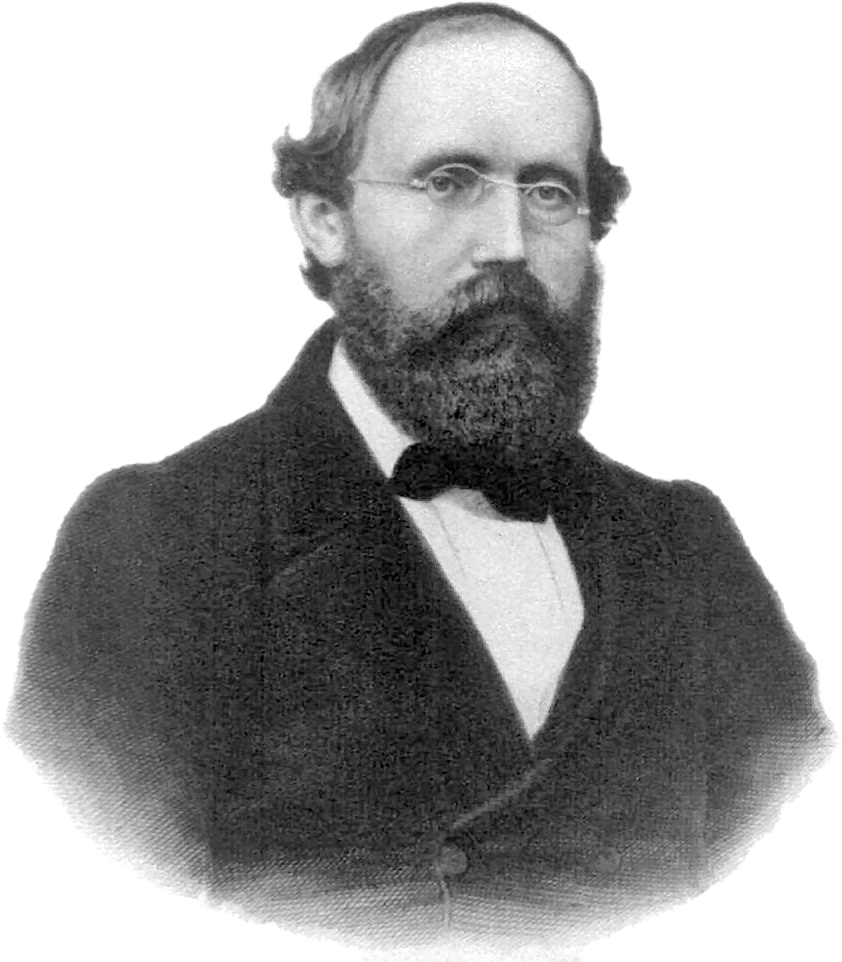
\includegraphics[width=0.15\textwidth]{images/riemann.png} \\
\emph{B.\xspace Riemann}
  \end{center}
\end{wrapfigure}

A Riemann sum (Bernhard Riemann, 17 September 1826--20 July 1866) is an
approximation of a definite integral by a finite sum. The sum is calculated by
partitioning the region into shapes (rectangles, trapezoids, parabolas, or
cubics) that together form a region that is similar to the region being
measured, then calculating the area for each of these shapes, and finally
summing these small areas. This approach can be used to find a numerical
approximation for a definite integral even if the fundamental theorem of
calculus does not make it easy to find a closed-form solution.

Because the region filled by the small shapes is usually not exactly the
same shape as the region being measured, the Riemann sum will differ
from the area being measured. This error can be reduced by dividing up
the region more finely, using smaller and smaller shapes. As the shapes
decrease in size, the sum approaches the value of the integral.

The left Riemann sum approximates $f$ by its value at the
left-end point gives multiple rectangles with base $\Delta x$ and height
$f(a + i\Delta x)$. Doing this for $i = 0, 1, \ldots , n-1$, and summing
the resulting areas gives
$$
A_\text{left} =
\Delta x \left[f(a) + f(a + \Delta x) + f(a+ 2 \, \Delta x)+ \cdots+f(b - \Delta x)\right].
$$
The left Riemann sum overestimates if $f$ is
\emph{monotonically decreasing} on this interval, and underestimates
if it is \emph{monotonically increasing}.

The right Riemann sum approximates $f$ by its value at the
right end-point. This gives
multiple rectangles with base $\Delta x$ and height $f(a + i\Delta x)$.
Doing this for $i = 1, \ldots, n$, and summing the resulting areas
produces
$$
A_\text{right} = \Delta x \left[ f( a
+ \Delta x ) + f(a + 2 \, \Delta x)+\cdots+f(b) \right].
$$
The right Riemann sum underestimates if $f$ is
monotonically decreasing, and overestimates if it is monotonically
increasing.

The \emph{midpoint rule} approximates $f$ at the midpoint of intervals, giving
$f(a + \tfrac{\Delta x}{2})$ for the first interval, for the next one
$f(a + 3\tfrac{\Delta x}{2})$, and so on until $f(b-\tfrac{\Delta
x}{2})$. Summing up the areas gives
$$
A_\text{mid} = \Delta x\left[f \left(a +
\tfrac{\Delta x}{2} \right) + f \left(a + \tfrac{3\,\Delta x}{2}
\right) + \cdots+f \left(b-\tfrac{\Delta x}{2} \right)\right].
$$

Refer to Figures \ref{figure:riemann-sin} and \ref{figure:riemann-cos}
for example plots of Riemann sums.

\begin{figure}[bth]
  \begin{centering}
    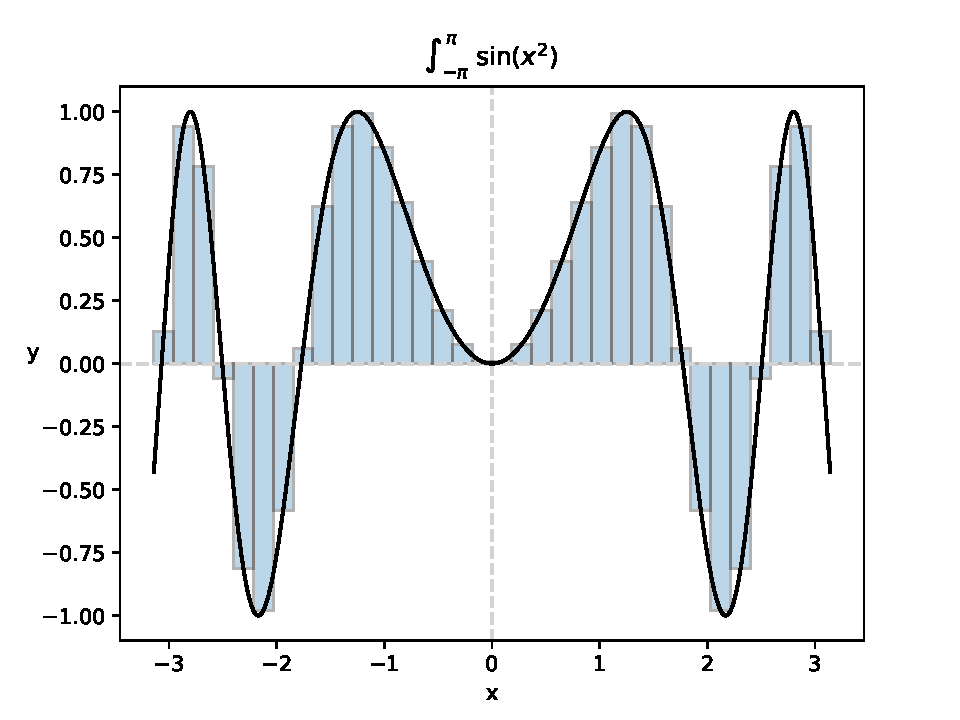
\includegraphics[width=0.65\textwidth]{riemann/sin.pdf}
    \caption{Midpoint Riemann sum for $\sin(x^2)$ over the range $[-\pi,
    \pi]$ with 50 partitions.}\label{figure:riemann-sin}
  \end{centering}
\end{figure}

\begin{figure}[bth]
  \begin{centering}
    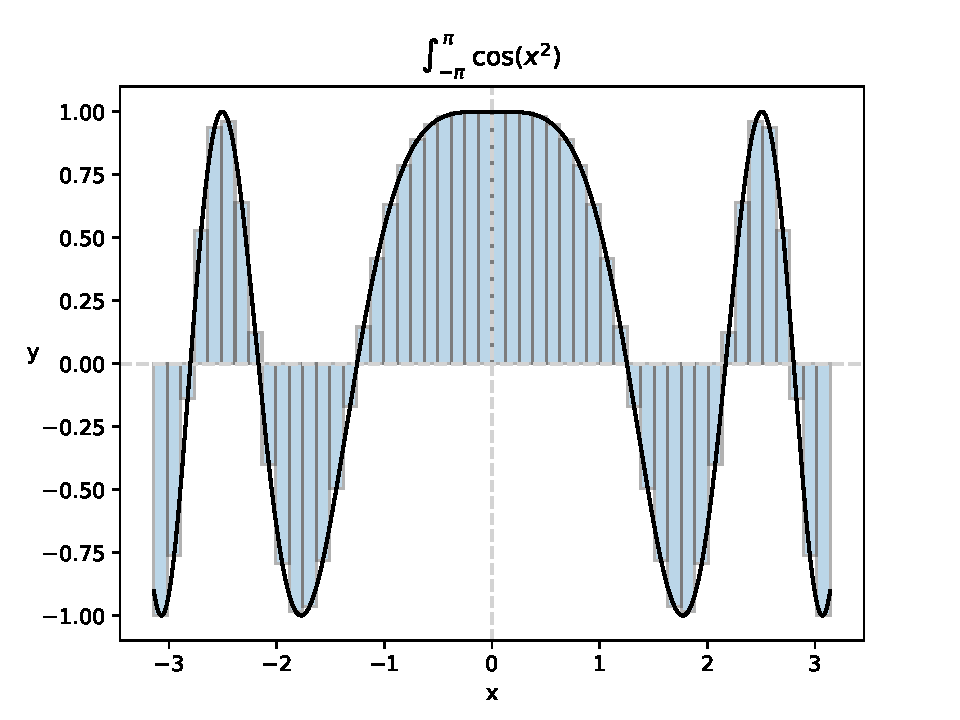
\includegraphics[width=0.65\textwidth]{riemann/cos.pdf}
    \caption{Midpoint Riemann sum for $\cos(x^2)$ over the range $[-\pi,
    \pi]$ with 50 partitions.}\label{figure:riemann-cos}
  \end{centering}
\end{figure}

\subsection{The Trapezoidal Rule}

The \emph{trapezoidal rule} (also known as the \emph{trapezoid rule}) is an
example of a closed Newton-Cotes quadrature. In numerical analysis,
this is a common technique for approximating a \emph{definite integral}.

It is assumed that the value of a function $f$ defined on $[a,b]$
is known at $n+1$ equally spaced points: $a \leq x_0 < x_1 < \dots
< x_n \leq b$. It is a form of \emph{closed} Newton–Cotes quadrature where
$x_0 = a$ and $x_n = b$, using
the function values at the interval end-points.
Newton–Cotes formulas using $n+1$ points can be
defined as
$$\int_a^b f(x) \,dx \approx \sum_{i=0}^n w_i\, f(x_i)$$
where $x_i = a + i h$, with
$h = (b-a)/n$.

The number $h$ is called \emph{step size}, $w_i$ are called \emph{weights}. The
weights can be computed as the integral of Lagrange basis polynomials, but you
do not need to worry about those here. Just know that they depend only on $x_i$
and not on the function $f$.

The trapezoidal rule works by approximating the region under the graph
of the function $f(x)$ as a trapezoid and calculating its area. It
follows that
$$
\int_{a}^{b} f(x) \, dx \approx \frac{b-a}{2} \left( f(a)+f(b) \right).
$$

The trapezoidal rule may be viewed as the result obtained by averaging
the left and right Riemann sums. The
integral can be even better approximated by partitioning the integration
interval, applying the trapezoidal rule to each subinterval, and summing
the results. In practice, this \emph{composite}
trapezoidal rule is usually what is meant by ``integrating with the
trapezoidal rule.'' Let $\{x_k\}$ be a partition of $[a,b]$ such that
$a=x_0 < x_1 < \cdots < x_{n-1} < x_n = b$ and $\Delta x_k$ be the
length of the $k^\text{th}$ subinterval (that is, $\Delta x_k = x_k -
x_{k-1}$), then
$$
\int_a^b f(x) \, dx \approx \sum_{k=1}^n \frac{f(x_{k-1}) + f(x_k)}{2} \Delta x_k.
$$

When the partition has a regular spacing,
when all the $\Delta x_k$ have the same value $\Delta x,$ the formula
can be simplified for calculation efficiency by factoring $h=\Delta x$
out:
\begin{align*}
\int_a^b f(x) \, dx & \approx \frac{h}{2}
\left(f(x_0) + 2f(x_1) + 2f(x_2) + 2f(x_3) + 2f(x_4) + \cdots +
2f(x_{n-1}) + f(x_n)\right) \\
& = \frac{h}{2}
\left(f(x_0) + 2\sum_{i=1}^{n-1} f(x_i) + f(x_n)\right).
\end{align*}
As $n$ increases, $h$ decreases, and as the resolution of the
partition increases the approximation becomes more accurate.

If we assume a fixed size $h = (b - b)/n$, then it is simple to
write the code for the trapezoid rule.

\begin{pylisting}{Implementation of the trapezoidal rule}
def trapezoid(f, a, b, n):
    h = (b - a) / n
    sum = f(a) + f(b)
    for j in range(1, n):
        sum += 2.0 * f(a + j * h)
    sum *= h / 2.0
    return sum
\end{pylisting}

\subsection{Simpson's Rules}


\begin{wrapfigure}{r}{0.11\textwidth}
  \begin{center}
  
\includegraphics[width=0.10\textwidth]{images/homer.png}\\
          \emph{H.\xspace Simpson}
  \end{center}
\end{wrapfigure}
We can do better than using the simple trapezoidal rule by adopting one of
Simpson's Rules  for approximating definite
integrals. Thomas Simpson (1710--1761) was a self-taught mathematician who supported himself
during his early years as a weaver. His primary interest was probability theory,
although in 1750 he published a two-volume calculus book entitled \emph{The
Doctrine and Application of Fluxions}. In German and some other languages, the
simplest of these rules is named after Johannes Kepler, who derived it in 1615
after seeing it used for wine barrels (\emph{Keplersche Fassregel}\,). The
approximate equality in the rule becomes exact if $f$ is a polynomial up to
$3^\text{rd}$ degree.

Interpolation with polynomials evaluated at equally spaced points in $[a,b]$
yields a Newton–Cotes formulas, of which the \emph{rectangle rule} and the
\emph{trapezoidal rule} are examples. Simpson's rule, which is based on a
polynomial of order 2, is also a Newton–Cotes formula.

\subsubsection{Simpson's 1/3 Rule}

Simpson's 1/3 rule is also an instance of a Newton-Cotes quadrature formula.
If the interval of integration $[a, b]$ is in some sense \emph{small},
then Simpson's rule with $n = 2$ subintervals will provide an
adequate approximation to the exact integral. By small we mean that
the function being integrated is relatively smooth over the interval
$[a, b]$. For such a function, a smooth quadratic interpolant like
the one used in Simpson's rule will give good results:

$$
\int_a^b f(x) \, dx \approx \frac{b - a}{6} \left[f(a) + 4f\left(\frac{a + b}{2}\right) + f(b)\right].
$$

\subsubsection{Composite Simpson's 1/3 Rule}\label{section:compositesimpson}

It is often the case that the function we are trying to integrate is not smooth
over the interval. Typically, this means that either the function is highly
oscillatory or lacks derivatives at certain points. One common way of handling
this problem is by breaking up the interval $[a, b]$ into $n > 2$ small
subintervals. Simpson's rule is then applied to each subinterval, with the
results being summed to produce an approximation for the integral over the
entire interval. This approach is termed the \emph{Composite Simpson's 1/3
rule}.

Suppose that the interval $[a, b]$ is split up into $n$ sub-intervals,
with $n$ an even number. Then, the composite Simpson's 1/3 rule is given by
\begin{align*}
  \int_a^b f(x) \, dx &\approx \frac{h}{3}
   \sum_{j=1}^{n/2}\big[f(x_{2j-2}) + 4f(x_{2j-1}) + f(x_{2j})\big] \\
  &= \frac{h}{3}
   \bigg[f(x_0) + 2\sum_{j=1}^{n/2-1} f(x_{2j}) + 4\sum_{j=1}^{n/2} f(x_{2j-1}) + f(x_n)\bigg],
 \end{align*}
where $x_j = a + jh$ for $j = 0, 1, \dots, n - 1, n$ with $h = (b -
a)/n$; in particular, $x_0 = a$ and $x_n = b$. The error when using the
composite Simpson's 1/3 rule is
$$
-\frac{h^4}{180} (b - a)f^{(4)}(\xi),
$$
where $\xi$ is some number between $a$ and $b$, and $h = (b - a)/n$ is
the step length.

\subsection{High Order Formul\ae}

These are not the only closed Newton-Cotes quadratures used for
numerical integration. For example, there is the composite Simpson's 3/8 rule:
 \begin{align*}
  \int_a^b f(x) \, dx &\approx \frac{3h}{8} \big[f(x_0) + 3f(x_1) + 3f(x_2) + 2f(x_3) + 3f(x_4) + 3f(x_5) + 2f(x_6) + {} \\
  &\qquad\qquad \cdots + 3f(x_{n-2}) + 3f(x_{n-1}) + f(x_n)\big] \\
  &= \frac{3h}{8} \left[f(x_0) + 3 \sum_{i \ne 3k}^{n-1} f(x_i) + 2 \sum_{j=1}^{n/3 - 1} f(x_{3j}) + f(x_n) \right] \quad \text{for  } k \in \mathbb{N}_0.
 \end{align*}
It has a smaller error term of
$$
 -\frac{h^4}{80} (b - a)f^{(4)}(\xi),
$$
but can only be used  this if $n$ is a \emph{multiple of three}.

Simpson's 3/8 rule is more difficult to implement directly, since it is not
obvious how we write a loop for the first summation. Instead, we ask what that
summation actually means: it means sum for all indices that are not multiples of
$3$ and the second summation for multiples of $3$. The code then follows easily.

\begin{pylisting}{Implementation of composite Simpson's 3/8 rule}
def simpson_38(f, a, b, n):
    h = (b - a) / n
    sum = f(a) + f(b)
    for i in range(1, n):
        if i % 3 != 0:
            sum += 3 * f(a + i * h)
        else:
            sum += 2 * f(a + i * h)
    sum *= h * 3 / 8
    return sum
\end{pylisting}

And, finally, there is the composite Boole's rule.
Yes, that George Boole (2 November 1815--8 December 1864), the founder of Boolean logic.
Boole's rule is also a Newton-Cotes formula with a decreased error term. In order to use Boole's composite rule, the number of partitions should be a multiple of 12.
$$
  \int_{a}^{b} f(x)\,dx
  = \frac{2 h}{45}
    \left(
         7(f(x_0) + f(x_n))
      + 32\left(\sum_{i \in \{1, 3,  \ldots, n-1\}} f(x_i)\right)
      + 12\left(\sum_{i \in \{2, 6,  \ldots, n-2\}} f(x_i)\right)
      + 14\left(\sum_{i \in \{4, 8,  \ldots, n-4\}} f(x_i)\right)
    \right)
$$
that has the error term
$$
-\,\frac{8}{945} h^7 f^{(6)}(\xi) .
$$

The formula for Boole's rule might appear daunting, but the code is not too bad.
It just requires a little thought. Again, you ask, ``What does each summation
do?''

\begin{pylisting}{Implementation of Boole's rule}
def boole(f, a, b, n):
    h = (b - a) / n
    sum = 7 * (f(a) + f(b))
    for i in range(1, n, 2):     sum += 32 * f(a + i * h)
    for i in range(2, n - 1, 4): sum += 12 * f(a + i * h)
    for i in range(4, n - 3, 4): sum += 14 * f(a + i * h)
    sum *= h * 2 / 45
    return sum
\end{pylisting}

If you are intrigued by these and other numerical computations, then we
encourage you to do some reading on you own, or take a course in the Applied
Mathematics department.

\begin{itemize}
  \item Burden, Richard L., and J. Douglas Faires. \emph{Numerical Analysis},
  $7^\text{th}$ edition, 2001. Thomson Learning ISBN 0-534-38216-9.
  \item Abramowitz, Milton, and Irene A. Stegun, \emph{eds}. \emph{Handbook of
    mathematical functions with formulas, graphs, and mathematical tables}. Vol.
    55. US Government printing office, 1970.
\end{itemize}

\section{Taylor Series}

\epigraphwidth=0.75\textwidth
\epigraph{\emph{Let us change our traditional attitude to the construction of
programs. Instead of imagining that our main task is to instruct a computer what
to do, let us concentrate rather on explaining to human beings what we want a
computer to do.}} {---Donald Knuth}

\noindent As we know, computers are simple machines that carry out a sequence of
very simple steps, albeit very quickly. Unless you have a special-purpose
processor, a computer can only compute \emph{addition}, \emph{subtraction},
\emph{multiplication}, and \emph{division}. If you think about it, you will see
that the functions that might interest you when dealing with real or complex
numbers can be built up from those four operations.  We use many of these
functions in nearly every program that we write, so we ought to understand how
they are created.

If you recall from your calculus class, with some conditions a function $f(x)$
can be represented by its Taylor series (Brook Taylor, 18 August 1685--29 December 1731)
expansion near some point $a$:
\[
  f(x) = f(a) + \sum_{k=1}^\infty \frac{f^{(k)}(a)}{k!}{(x-a)}^k.
\]
\textcolor{red}{Note: when you see $\Sigma$ with definite limits, you should generally think of a
\texttt{for} loop.}

Since we cannot compute an infinite series, we must be content to calculate a
finite number of terms. In general, the more terms that we compute, the more
accurate our approximation.

For example, if we expand to $10$ terms we get:
\begin{align*}
  f(x) = f(a) &+ \taylorterm{1} + \taylorterm{2} + \taylorterm{3} + \taylorterm{4} \\
              &+ \taylorterm{5} + \taylorterm{6} + \taylorterm{7} + \taylorterm{8} \\
              &+ \taylorterm{9} + \operatorname{O}({(x-a)}^{10}). \\
\end{align*}
In the case $a =0$, then it is called a \emph{Maclaurin series}.  Often we
choose $0$ since it is simpler, but the closer to the value of $x$ the better we
will approximate the function. \textcolor{red}{Note: $k! =
k(k-1)(k-2)\times...\times1$, and by definition, $0! = 1$. }

What is the $\operatorname{O}\left((x-a)^{10}\right)$ term? That is the \emph{error term} that
is ``on the order of'' the value in parentheses. This is different from the
\emph{big-O} that we will discuss with regard to algorithm analysis.

The number $e$, also known as \emph{Euler's number} (Leonhard Euler,
1707--1783), is an irrational mathematical constant approximately equal to
$2.71828$, that appears pervasively in the natural and mathematical worlds. It
is the base of the natural logarithm, it is the limit of
$\lim_{n\rightarrow\infty} (1 + \frac{1}{n})^n$ which was discovered by Jacob
Bernoulli (6 January 1655--16 August 1705) in his work on the calculation of
compound interest.

The function $f(x)=e^x$ is a very attractive function, since $f^{(k)}(x) = f^{(k-1)}(x) = \cdots = f^\prime(x) = f(x) = e^x$.
This is one of the simplest series when centered at $0$, since $e^0 = 1$.
\begin{align*}
  e^x & = \sum_{k=0}^{\infty} \frac{x^k}{k!} = 1 + \mlterm{1} + \mlterm{2} +
  \mlterm{3} + \mlterm{4} + \mlterm{5} + \mlterm{6} + \mlterm{7} + \mlterm{8} +
  \mlterm{9} + \ldots
\end{align*}

\section{\LARGE $e^x$}\label{section:exp}

We have a nice series for $e^x$ that converges quickly. In
Figure~\ref{figure:exp}, we use our expansion to $10$ terms and plot for
$e^x, x=0,\ldots,{10}$. We see that the approximation starts to diverge
significantly around $x = 7$. What this tells us is that $10$ terms are
insufficient for an accurate approximation, and more terms are needed.

\begin{figure}[bth]
  \begin{centering}
    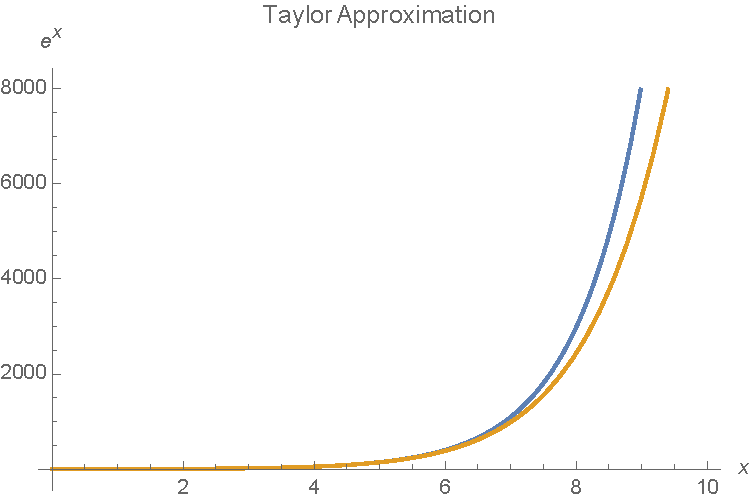
\includegraphics[width=0.65\textwidth]{images/exp.pdf}
    \caption{Comparing $e^x$ with its 10-term Taylor approximation
    centered at zero.}\label{figure:exp}
  \end{centering}
\end{figure}

\begin{figure}[bth]
  \begin{centering}
    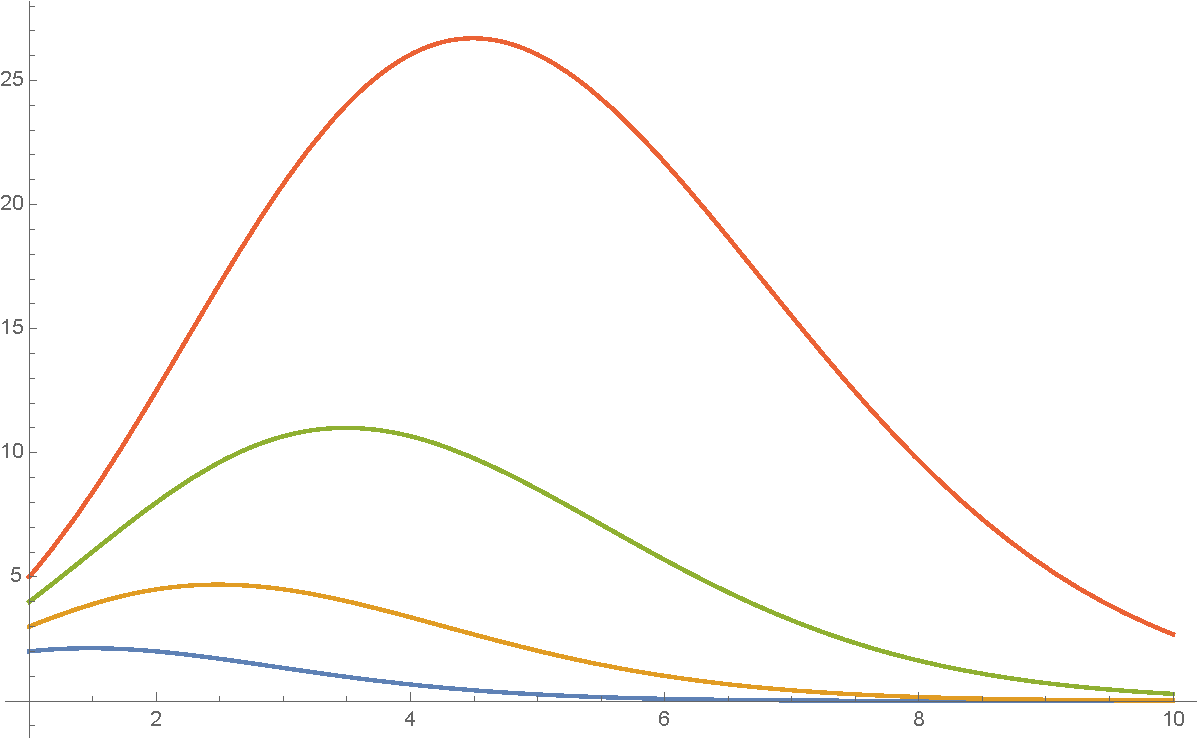
\includegraphics[width=0.75\textwidth]{images/growth.pdf}
    \caption{Comparing $\dfrac{x^k}{k!}$ for $x=2,3,4,5$.}\label{figure:growth}
  \end{centering}
\end{figure}

If we are na\"ive about computing the terms of the series we can quickly
get into trouble --- the values of $k!$ get large \emph{very quickly}.
We can do better if we observe that:
$$
\frac{x^k}{k!} = \frac{x^{k-1}}{(k-1)!} \times \frac{x}{k} .
$$

At first, that looks like a recursive definition (and in fact, you could
write it that way, but it would be wasteful). As we progress through the
computation, assume that we know the previous result. We then just have
to compute the next term and multiply it by the previous term.  At each
step we just need to compute $\frac{x}{k}$, starting with $k = 0!=1$
and multiply it by the previous value and add it
into the total. It turns into a simple \texttt{for} or \texttt{while}
loop.

We can use an $\epsilon$ (epsilon) to halt the computation since $|x^k| \ll k!$
for a sufficiently large $k$. Consider Figure \ref{figure:growth}: $x^k$
dominates briefly but is quickly overwhelmed by $k!$ and so the ratio rapidly
approaches zero. The following is an approximation of $e^x$ implemented in
Python which halts computation at a default epsilon $\epsilon = 10^{-14}$.
Make note of the efficient iterative computation of $x^k/k!$.

\begin{pylisting}{Implementation of $e^x$}
def exp(x, epsilon = 1e-14):
    trm = 1.0
    sum = trm
    k = 1
    while trm > epsilon:
        trm *= abs(x) / k
        sum += trm
        k += 1
    return sum if x > 0 else 1 / sum
\end{pylisting}

We take a different approach for $x<0$ by noting that $e^{-x} = 1/e^x$. Why is
that necessary? The series for $x\ge 0$ has all positive terms and so converges
quickly, but for $x < 0$ it is an \emph{alternating series} and converges much
more slowly. Consequently, we do a little algebra and our computation is much
more efficient.

\section{Sine and Cosine}\label{section:sincos}

The sine and cosine functions repeat over the interval $[-2\pi, 2\pi]$. That is,
$\sin(x)=\sin(x +2k\pi)$ and $\cos(x)=\cos(x +2k\pi)$ for every integer $k$.
Centering their series around $0$ makes computation simpler and more efficient.

The Taylor series for $\sin(x)$
centered about $0$ is:
$$
\sin(x)= \sum_{k=0}^{\infty} (-1)^k \frac{x^{2k + 1}}{(2k +1)!}.
$$
If we expand a few terms, then we get:
$$
  \sin(x) = x - \mlterm{3} + \mlterm{5} - \mlterm{7} + \mlterm{9} - \mlterm{11}
              + \mlterm{13} + \operatorname{O}(x^{14}).
$$

We can implement this series as a simple loop. We will continue the loop until
the last term is less than the error we have agreed is acceptable. Why not loop
until it reaches \emph{zero}? Think about it: $\texttt{float} \ne {\mathbb R}$.

\begin{pylisting}{Implementation of $\sin(x)$}
def sin(x, epsilon = 1e-14):
    s, v, t, k = 1.0, x, x, 3.0
    while abs(t) > epsilon:
        t = t * (x * x) / ((k - 1) * k)
        s = -s
        v += s * t
        k += 2.0
    return v
\end{pylisting}

The series for $\cos(x)$ centered about $0$ is:
$$
\cos(x)= \sum_{k=0}^{\infty} (-1)^k \frac{x^{2k}}{(2k)!} .
$$
If we expand a few terms, then we get:
$$
  \cos(x) = 1 - \mlterm{2} + \mlterm{4} - \mlterm{6} + \mlterm{8} - \mlterm{10}
              + \mlterm{12} + \operatorname{O}(x^{14}).
$$

\section{Square Roots and Logarithms}\label{section:sqrtlog}

Can we just use the Taylor series to compute square root and the natural
logarithm? Consider that $\sqrt{x} = x^\frac{1}{2}$, and so it is
already a series but it has just \emph{one term}. If we attempt a Taylor series we see that
$$
\frac{d}{dx} \sqrt{x} = \frac{1}{2 \sqrt{x}}
\quad\text{and}\quad \frac{d^2}{dx^2} \sqrt{x} = -\frac{1}{4 x^{3/2}}
\quad\text{and}\quad \frac{d^3}{dx^3} \sqrt{x} = \frac{3}{8 x^{5/2}} \quad\ldots
$$
all of which contain $\sqrt{x}$, thus doing us no good at all.
How about a series for
$\log(x)$? Since $\log(0)$ is undefined, we will use $\log(x+1)$:
$$
\log(x+1) =
x-\frac{x^2}{2}+\frac{x^3}{3}-\frac{x^4}{4}+\frac{x^5}{5}-\frac{x^6}{6}+\frac{x^7}{7}+O\left(x^8\right).
$$
It exists, but it converges \emph{extremely slowly}.

To compute $\sqrt{x}$ and $\log(x)$, you will use Newton's method,
also called the Newton-Raphson method. It is an iterative algorithm
to approximate roots of real-valued functions:
solving $f(x) = 0$. Each iteration $k+1$ of Newton's method produces
successively better approximation:
\[
  x_{k+1} = x_k - \frac{f(x_k)}{f'(x_k)} .
\]

For example, consider computing $\sqrt{y}$  with Newton's method. That
is, in order to solve for some $\sqrt{y}$, we are searching for a \emph{non-negative} $x$
such that $x^2 = y$. We can express this as finding the root of $f(x) = x^2 -
y$, giving us:
\[
  x_{k+1} = x_k - \frac{x_k^2-y}{2x_k} = \frac{y}{2 x_k}+\frac{x_k}{2} = \frac{1}{2}\left( x_k + \frac{y}{x_k} \right).
\]
Each guess $x_{k+1}$ gives a successive improvement over the previous guess
$x_k$. Your function \texttt{Sqrt()} should behave the same as \texttt{log()}
from \texttt{<math.h>}: compute $\sqrt{x}$. The following is an example that
implements Newton's method for computing square roots.

\begin{pylisting}{Implementation of $\sqrt{x}$}
def sqrt(x, epsilon = 1e-14):
    z = 0.0
    y = 1.0
    while abs(y - z) > epsilon:
        z = y
        y = 0.5 * (z + x / z)
    return y
\end{pylisting}

Your function \texttt{Log()} should behave the same as \texttt{log()} from
\texttt{<math.h>}: compute $\log(x)$ ($\ln(x)$). The procedure is very much the
same as it was for the square root example, the main difference being that $f(x)
= y - e^x$, since $e^x$ is the inverse of $\log$, \textit{i.e.} $\log(e^x) = x$.
Another key difference is the value converges when $e^{x_{i}} - y$ is small,
where $x_0$ is initially $1.0$ and is used to compute better approximations. In
order to implement this function, you will have to use your \texttt{Exp()}
function.

\begin{pylisting}{Implementation of $\log(x)$}
def log(x, epsilon = 1e-14):
    y = 1.0
    p = exp(y)
    while abs(p - x) > epsilon:
        y = y + x / p - 1
        p = exp(y)
    return y
\end{pylisting}

\subsection{Scaling}
You can implement the $\log(x)$ and $\sqrt{x}$ functions directly, and if you do
you will find that they work well for small $x$ but fail when $x$ increases. For
$\sqrt{x}$ the algorithm is simply less efficient, but for $\log(x)$ it will
fail for $x> 29$ due to floating-point numbers not being real numbers. What
should we do? The answer is surprisingly simple: we scale the problem to a small
interval.

In the case of $\sqrt{x}$ we will factor out all powers of \emph{four}:
let $x = 4^k \times a $. This is trivially true for $k=0$, and you will
see that it can be done for $k\ge 1$ if $x\ge 4$. Suppose $x=48$, then
$x = 4^2\times 3$, with $a=3$. Observe that $\sqrt{4^k a} =
2^k\sqrt{a}$. For every $4$ that we factor out, we multiply by $2$
after we have computed the $\sqrt{a}$. In our example,
$\sqrt{48} = \sqrt{4^2\times 2} = 2^2\sqrt{3}= 4\sqrt{3}$. Why $4$? Four is a
\emph{perfect square}, so it is easier.

\begin{pylisting}{}
f = 1.0 # 2^0
while x > 1:
    x /= 4.0
    f *= 2.0 # 2^(k+1)
\end{pylisting}

In the case of $\log(x)$ observe that $\log(x) = \log(a\times e^f
) = \log(a) + \log(e^f)  = f + \log(a)$ when $x = e^f\times a$. We factor out $e$, and
each time add $1$ to $f$ until $a<e$. This allows us to search for
$\log(a)$ over the small interval $[1, e)$.  For example, to calculate
$\log(917) \approx \log(e^7 \times 0.836195762413492) \approx 7 +
\log(0.836195762413492) \approx 6.821107472256466$.

\begin{pylisting}{}
e = 2.7182818284590455 # Euler's constant
while x > e:
    x /= e
    f += 1.0
\end{pylisting}

\section{Your Task}

\epigraphwidth=0.5\textwidth
\epigraph{\emph{The people will believe what the media tells them they
believe.}}{---George Orwell}

\noindent
\begin{itemize}
  \item Initialize your Bloom filter and hash table.
  \item Read in a list of \emph{badspeak} words with \texttt{fscanf()}.
    Again, badspeak is simply oldspeak without a newspeak translation.
    Badspeak is strictly forbidden. Each badspeak word should be added
    to the Bloom filter and the hash table. The list of proscribed words
    will be in \texttt{badspeak.txt}, which can be found in the
    \texttt{resources} repository.
  \item Read in a list of \emph{oldspeak} and \emph{newspeak} pairs with
    \texttt{fscanf()}. Only the oldspeak should be added to the Bloom
    filter. The oldspeak \emph{and} newspeak are added to the hash
    table. The list of oldspeak and newspeak pairs will be in
    \texttt{newspeak.txt}, which can also be found in the
    \texttt{resources} repository.
  \item Now that the lexicon of badspeak and oldspeak/newspeak
    translations has been populated, you can start to filter out words.
    Read words in from \texttt{stdin} using the supplied parsing module.
  \item For each word that is read in, check to see if it has been added
    to the Bloom filter. If it has not been added to the Bloom filter,
    then no action is needed since the word isn't a proscribed word.
  \item If the word has most likely been added to the Bloom filter,
    meaning \texttt{bf\_probe()} returned \texttt{true}, then further
    action needs to be taken.
    \begin{enumerate}
      \item If the hash table contains the word and the word \emph{does
        not} have a newspeak translation, then the citizen who used this
        word is guilty of \texttt{thoughtcrime}. Insert this badspeak
        word into a list of badspeak words that the citizen used in
        order to notify them of their errors later. What data structure
        could be used to store these words?
      \item If the hash table contains the word, and the word \emph{does}
        have a newspeak translation, then the citizen requires
        counseling on proper \emph{Rightspeak}. Insert this oldspeak
        word into a list of oldspeak words with newspeak translations in
        order to notify the citizen of the revisions needed to be made
        in order to practice Rightspeak.
      \item If the hash table does not contain the word, then all is
        good since the Bloom filter issued a false positive. No
        disciplinary action needs to be taken.
    \end{enumerate}
  \item If the citizen is accused of thoughtcrime \emph{and} requires
    counseling on proper \emph{Rightspeak}, then they are given a
    reprimanding \emph{mixspeak message} notifying them of their
    transgressions and promptly sent off to \emph{joycamp}. The message
    should contain the list of badspeak words that were used followed by
    the list of oldspeak words that were used with their proper newspeak
    translations.

  \begin{shlisting}{}
Dear beloved citizen of the GPRSC,

We have some good news, and we have some bad news.
The good news is that there is bad news. The bad news is that you will
be sent to joycamp and subjected to a week-long destitute existence.
This is the penalty for using degenerate words, as well as using
oldspeak in place of newspeak. We hope you can correct your behavior.

Your transgressions, followed by the words you must think on:

kalamazoo
antidisestablishmentarianism
write -> papertalk
sad -> happy
read -> papertalk
music -> noise
liberty -> badfree\end{shlisting}

  \item If the citizen is accused solely of thoughtcrime, then they are
    issued a thoughtcrime message and also sent off to \emph{joycamp}.
    The \emph{badspeak message} should contain the list of badspeak
    words that were used.

  \begin{shlisting}{}
Dear beloved citizen of the GPRSC,

You have been caught using degenerate words that may cause
distress among the moral and upstanding citizens of the GPSRC.
As such, you will be sent to joycamp. It is there where you will
sit and reflect on the consequences of your choice in language.

Your transgressions:

kalamazoo
antidisestablishmentarianism\end{shlisting}

  \item If the citizen only requires counseling, then they are issued an
    encouraging \emph{goodspeak message}. They will read it, correct
    their \emph{wrongthink}, and enjoy the rest of their stay in the
    GPRSC. The message should contain the list of oldspeak words that
    were used with their proper newspeak translations.

    \begin{shlisting}{}
Dear beloved citizen of the GPRSC,

We recognize your efforts in conforming to the language standards
of the GPSRC. Alas, you have been caught uttering questionable words
and thinking unpleasant thoughts. You must correct your wrongspeak
and badthink at once. Failure to do so will result in your deliverance
to joycamp.

Words that you must think on:

write -> papertalk
sad -> happy
read -> papertalk
music -> noise
liberty -> badfree\end{shlisting}

  \item Each of the messages are defined for you in \texttt{messages.h}.
    \textcolor{red}{You may not modify this file}.

  \item The list of the command-line options your program must support
    is listed below. \emph{Any} combination of the command-line options
    must be supported.
    \begin{itemize}
      \item \texttt{-h} prints out the program usage. Refer to the
      reference program in the resources repository for what to print.
      \item \texttt{-t size} specifies that the hash table
        will have \texttt{size} entries (the default will be $2^{16}$).
      \item \texttt{-f size} specifies that the Bloom filter
        will have \texttt{size} entries (the default will be $2^{20}$).
      \item \texttt{-s} will enable the printing of statistics to
        \texttt{stdout}. The statistics to calculate are:
        \begin{itemize}
          \item Average binary search tree size
          \item Average binary search tree height
          \item Average branches traversed
          \item Hash table load
          \item Bloom filter load
        \end{itemize}
        The latter three statistics are computed as follows:
        \begin{align*}
          \text{Average branches traversed} &=
          \frac{\texttt{branches}}{\texttt{lookups}} \\
          \text{Hash table load} &= 100 \times \frac{\texttt{ht\_count()}}{\texttt{ht\_size()}} \\
          \text{Bloom filter load} &= 100 \times \frac{\texttt{bf\_count()}}{\texttt{bf\_size()}}
        \end{align*}
        The hash table load and Bloom filter load should be printed with
        up to 6 digits of precision. \textcolor{red}{Enabling the
        printing of statistics should \emph{suppress all messages} the
        program may otherwise print.} The number of lookups is defined
        as the number of times \texttt{ht\_lookup()} and
        \texttt{ht\_insert()} is called. The number of branches is
        defined as the count of links traversed during calls to
        \texttt{bst\_find()} and \texttt{bst\_insert()}. The global
        variable \texttt{lookups} should be defined in \texttt{ht.c} and
        the global variable \texttt{branches} should be defined in
        \texttt{bst.c}.
    \end{itemize}
\end{itemize}

\section{The Main Program}

\epigraphwidth=0.6\textwidth
\epigraph{\emph{A few dud universes can really clutter up your
basement.}} {---Neal Stephenson, \emph{In the Beginning\ldots Was the
Command Line}}

\noindent As stated in \S\ref{section:task}, you are expected to write a
dedicated program, \texttt{integrate}, that computes the numerical
integration of a function over a specified interval using the composite
Simpson's rule. This program, implemented in \texttt{integrate.c}, must
use \texttt{getopt()} and must accept the following command-line
options:

\begin{itemize}
  \item \textbf{\texttt{-a}} : Sets the function to integrate to
    $\sqrt{1 - x^4}$.
  \item \textbf{\texttt{-b}} : Sets the function to integrate to
    ${1}/{\log(x)}$.
  \item \textbf{\texttt{-c}} : Sets the function to integrate to
    $e^{-x^2}$.
  \item \textbf{\texttt{-d}} : Sets the function to integrate to
    $\sin(x^2)$.
  \item \textbf{\texttt{-e}} : Sets the function to integrate to
    $\cos(x^2)$.
  \item \textbf{\texttt{-f}} : Sets the function to integrate to
    $\log(\log(x))$.
  \item \textbf{\texttt{-g}} : Sets the function to integrate to
    ${\sin(x)}/{x}$.
  \item \textbf{\texttt{-h}} : Sets the function to integrate to
    ${e^{-x}}/{x}$.
  \item \textbf{\texttt{-i}} : Sets the function to integrate to
    $e^{e^x}$.
\item \textbf{\texttt{-j}} : Sets the function to integrate to $\sqrt{\sin^2(x) + \cos^2(x)}$.
  \item \textbf{\texttt{-n partitions}} : Sets the upper limit of
    partitions to use in the composite Simpson's rule to
    \texttt{partitions}. This should have a default value of 100.
  \item \textbf{\texttt{-p low}} : Sets the low end of the interval to
    integrate over to \texttt{low}. This \emph{should not} have a
    default value and must be specified each time the program is run.
  \item \textbf{\texttt{-q high}} : Sets the high end of the interval to
    integrate over to \texttt{high}. This \emph{should not} have a
    default value and must be specified each time the program is run.
  \item \textbf{\texttt{-H}} : Displays the program's usage and
    synopsis.
\end{itemize}

The functions you will integrate will be provided to you in the
\texttt{functions.c} file in the resources repository. Each function is
implemented using functions from \emph{your} math library, so be sure to finish
the library first.

You are given Table \ref{table:values}, as well as a working reference program
in the resources repository, for you to compare the results of your numerical
integrations against. Each function should be integrated using \emph{even}
numbered partitions from $2, 4, \ldots,n-2, n$, where $n$ is the specified upper
partition limit. The output of your program \emph{must} be formatted as follow:

\begin{shlisting}{}
$ ./integrate -a -p 0.0 -q 1.0 -n 10
sqrt(1 - x^4),0.000000,1.000000,10
2,0.812163891034571
4,0.852988388966857
6,0.862714108378597
8,0.866720323920874
10,0.868814915051592
\end{shlisting}

The first line of output should be
\texttt{<function>,<low>,<high>,<partitions>}. The subsequent lines
should be \texttt{<partition>,<value>}, where \texttt{value} is the
approximated integrated value. Commas should be used as the delimiting
character. This format will help you plot your results in your
assignment writeup.

\def\fz{\phantom{x}}
\begin{table}\label{fns}
  \centering
  \caption{Table of approximated values.}\label{table:values}
  \medskip
  \begin{tabular}{lrrr}
    \toprule
    \multicolumn{1}{c}{Integral} & \multicolumn{1}{c}{Low} &
    \multicolumn{1}{c}{High} & \multicolumn{1}{c}{Value} \\
    \midrule
    $\sqrt{1-x^4}$ & $0$ & $1$ & 0.87401918476405\fz\fz \\
    ${1}/{\log(x)}$ & $2$ & $3$ & 1.118424814549702\fz \\
    $e^{-x^2}$ & $-10$ & $10$ & 1.772453850905508\fz \\
    $\sin(x^2)$ & $-\pi$ & $\pi$ & 1.545303425380133\fz \\
    $\cos(x^2)$ & $-\pi$ & $\pi$ & 1.131387027213366\fz \\
    $\log(\log(x))$ & $2$ & $10$ & 3.952914142858876\fz \\
    ${\sin(x)}/{x}$& $-4\pi$ & $4\pi$ & 2.984322451168924\fz \\
    ${e^{-x}}/{x}$ & $1$ & $10$ & 0.2193797774265986 \\
    $e^{e^x}$ & $0$ & $1$ & 6.316563839027766\fz \\
    $\sqrt{\sin^2(x)+\cos^2(x)}$ & 0 & $\pi$ & 3.141592653589797\fz \\
    \bottomrule
  \end{tabular}
\end{table}

The values that you compute should be close to Table\xspace\ref{table:values}.
How close your approximations comes will depend on the number of intervals that
you select. \emph{Do not just choose a large number}. An important task in
numerical analysis is to understand what is necessary to gain the desired
accuracy. Indeed, if you make the number of intervals \emph{too large} you will
not only waste computing resources, but you may find that your accuracy
\emph{goes down}.

\section{Deliverables}

\epigraphwidth=0.4\textwidth
\epigraph{\emph{It is such a sweet temptation \\ It gives such grief relief \\
It is such a false sensation \\ How come that's so hard to believe?}}{---Ray
Wylie Hubbard, \emph{Loco Gringo's Lament}}

You will need to turn in the following source code and header files:

\begin{enumerate}
  \item Your program \emph{must} have the following source and header
    files:
  \begin{itemize}
    \item \texttt{universe.c} implements the \texttt{Universe} ADT.
    \item \texttt{universe.h} specifies the interface to the \texttt{Universe}
      ADT. This file is provided and \emph{may not} be modified.
    \item \texttt{life.c} contains \texttt{main()} and \emph{may}
      contain any other functions necessary to complete your implementation of
      the Game of Life.
  \end{itemize}
\end{enumerate}

You can have other source and header files, but \emph{do not try to be overly
clever}. You will also need to turn in the following:

\begin{enumerate}
  \item \texttt{Makefile}:
    \begin{itemize}
      \item \texttt{CC = clang} must be specified.
      \item \texttt{CFLAGS = -Wall -Wextra -Werror -Wpedantic} must be specified.
      \item \texttt{make} must build the \texttt{life} executable, as should
        \texttt{make all} and \texttt{make life}.
      \item \texttt{make clean} must remove all files that are compiler
        generated.
      \item \texttt{make format} should format all your source code,
        including the header files.
    \end{itemize}
  \item \texttt{README.md}: This must use proper Markdown syntax. It
    must describe how to use your program and \texttt{Makefile}. It
    should also list and explain any command-line options that your
    program accepts. Any false positives reported by \texttt{scan-build}
    should be documented and explained here as well. Note down any known
    bugs or errors in this file as well for the graders.
  \item \texttt{DESIGN.pdf}: This document \emph{must} be a proper
    PDF\@. This design document must describe your design and design
    process for your program with enough detail such that a sufficiently
    knowledgeable programmer would be able to replicate your
    implementation. \textcolor{red}{This does not mean copying your
    entire program in verbatim}. You should instead describe how your
    program works with supporting pseudocode.
  \item \texttt{WRITEUP.pdf}: This document \emph{must} be a proper
    PDF\@. This writeup document must include everything you learned from
    this assignment. Make sure to mention everything in detail while being as precise as possible. How well you explain all the lessons you have learned in this assignment will be really important here. 
\end{enumerate}

\section{Submission}

Refer back assignment 0 for the instructions on how to properly submit
your assignment through \texttt{git}. Remember: \emph{add},
\emph{commit}, and \emph{push}!

\textcolor{red}{Your assignment is turned in \emph{only} after you have
pushed and submitted the commit ID you want graded on Canvas. ``I
forgot to push'' and ``I forgot to submit my commit ID'' are not valid
excuses. It is \emph{highly} recommended to commit and push your changes
\emph{often}.}

\section{Supplemental Readings}

\epigraph{\emph{The more that you read, the more things you will know. The
more that you learn, the more places you'll go.}}{---Dr.\ Seuss}

\begin{itemize}
  \item \textit{The C Programming Language} by Kernighan \& Ritchie
  \begin{itemize}
    \item Chapter 7
    \item Appendix B
  \end{itemize}
  \item \textit{Introduction to Algorithms} by T.\ Cormen, C.\
    Leiserson, R.\ Rivest, \& C.\ Stein
    \begin{itemize}
      \item Chapter 31 \S 31.2, \S 31.3, \S 31.6, \S 31.7, \S 31.8
    \end{itemize}
\end{itemize}

\vfill\begin{center}
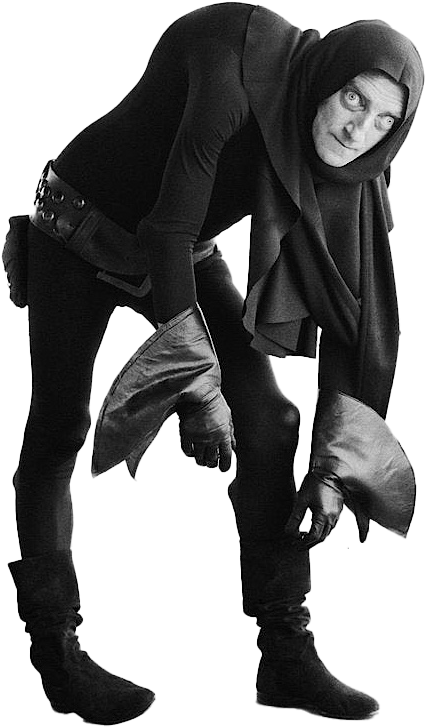
\includegraphics[height=1.75in]{images/marty-igor.png}
%\vspace{2\baselineskip}
\emph{In retrospect, come to think of it, isn't everything seen in retrospect?}
---Marty Feldman
\end{center}
\end{document}
